\subsection{Introducción}
Esta sección contiene los conceptos básicos para el diseño de una antena de tipo solenoide,
para aplicaciones RFID.
A lo largo de la guía se dan ejemplos para el cálculo de una antena con las siguientes
características:
\begin{itemize}
\item Alambre de cobre de 0.3mm de diámetro.
\item Número de espiras N = 5.
\item 0,05 m de diámetro interior.
\end{itemize}

\begin{figure}[H]
\centering
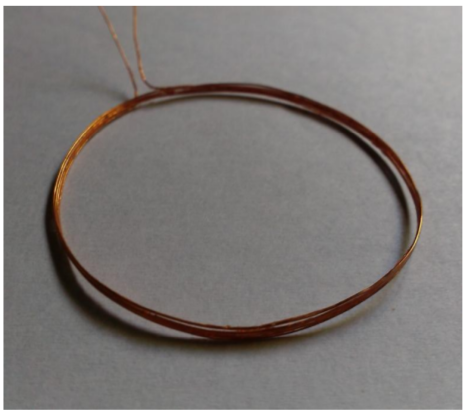
\includegraphics[scale=0.4]{antena/Antena.png}
\caption{Antena diseñada.}
\label{fig:antena}
\end{figure}

\subsection{Cálculo de la frecuencia de Resonancia}

\begin{figure}[H]
\centering
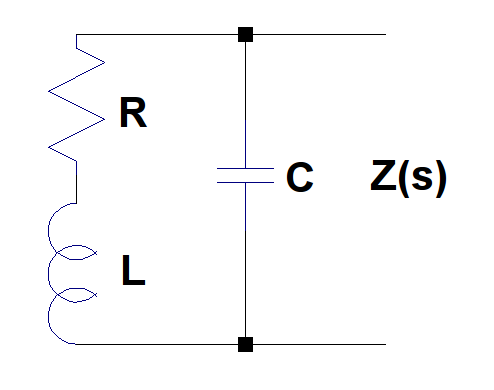
\includegraphics[scale=0.3]{antena/Antena_Equivalente.png}
\caption{Circuito de sintonía del PIC.}
\label{fig:antena_eq}
\end{figure}

El circuito muestra una impedancia:

\begin{equation}
Z(S) = \frac{LS + R}{LCS^2 + RCS + 1}
\end{equation}

Barriendo por el eje jω (S = jω) y multiplicando por el conjugado para separar la parte real
y la parte imaginaria:

$$Z(S)|_{S=j\omega} = \frac{j\omega L + R}{-LC\omega ^2 + j\omega RC + 1}$$
$$Z(S)|_{S=j\omega} = \frac{R + j\omega L}{(1 - LC\omega^2) + j\omega RC} * \frac{(1 - LC\omega ^2) - j(\omega RC)}{(1 - LC\omega ^2) - j(\omega)}$$
$$Z(j\omega) = \Omega + jX = \frac{R(1 - LC\omega ^2)-jR^2C\omega+j\omega L(1-LC\omega ^2)+\omega ^2 RLC}{(1 - LC\omega ^2)^2 - (RC\omega )^2}$$
$$Z(j\omega) = \Omega + jX = \frac{R(1 - LC\omega ^2)+\omega ^2RLC}{(1 - LC\omega ^2)^2 - (RC\omega )^2}+j\frac{\omega L(1 - LC\omega ^2)-R^2C\omega}{(1 - LC\omega ^2)^2 - (RC\omega )^2}$$

La frecuencia de resonancia se alcanza cuando la parte imaginaria de la impedancia se
hace nula, osea $X(j\omega _o) = 0$

$$X(j\omega _o) = \omega _o L(1 - LC\omega _o ^2)-R^2C\omega _o = 0$$
$$X(j\omega _o) = L(1 - LC\omega _o ^2)-R^2C = 0$$
\begin{equation}
\boxed{\omega _o = \sqrt[]{\frac{R ^2C - L}{L^2C}}}
\end{equation}

Para el diseño de una antena RFID, es necesario considerar el Q del inductor, ya que nos
interesa qué tan selectiva es la antena. Por definición $Q = \frac{\omega L}{R}$, siendo Q la selectividad del circuito resonante, \omega la frecuencia angular, L la inductancia y R la resistencia (pérdidas) de la antena.

\begin{figure}[H]
\centering
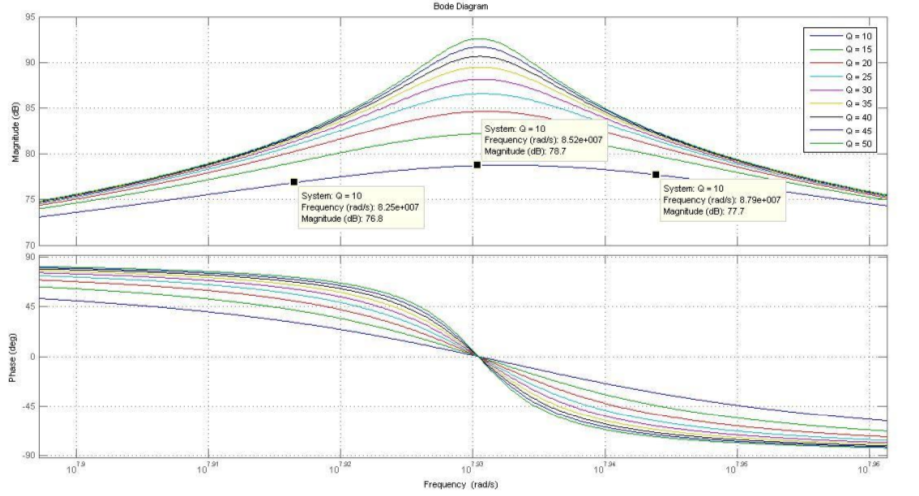
\includegraphics[scale=0.5]{antena/Respuesta_Frecuencia.png}
\caption{Respuesta en frecuencia del circuito de sintonía.}
\label{fig:transf_frec}
\end{figure}

Para la comunicación desde el PICC al PCD, se modula la portadora con ASK (modulación por desplazamiento de amplitud) a una frecuencia de 847 kHz. Esto nos produce, en el espectro, dos bandas laterales con respecto a la frecuencia central. En la figura \ref{fig:transf_frec} se ve que con un Q de 10, la respuesta cae aproximadamente 1 dB.
Si se aumenta el Q, el circuito se vuelve más selectivo, filtrando las bandas laterales y perdiendo así la modulación. 
Según \cite{antena_guide}, el factor de calidad debe ser:
\begin{equation}
\boxed{Q \leq \frac{f_c}{2B}}
\end{equation}
Siendo $f_c$ la frecuencia central (en este caso 13,56MHz) y B el ancho de banda. El Q
óptimo para la norma ISO 15693 es $9\leq Q\geq 16$.
Por lo tanto, para este diseño, se escoge un Q de 10.

\subsection{Tensión inducida en la bobina}
A partir de las leyes del magnetismo, se despeja la ecuación de la tensión inducida en una bobina:
\begin{equation}
V = -N\frac{d\phi}{dt}
\end{equation}
\begin{equation}
\phi = \int_{}^{}  B \, dS
\end{equation}
Suponiendo B, S y \psi constantes en el intervalo a analizar, se llega a la siguiente fórmula:
\begin{equation}
\boxed{V = 2 \pi fNBS\cos(\alpha)}
\end{equation}

Siendo f la frecuencia de trabajo, N el número de espiras, B la densidad de flujo magnético, S el área de la bobina y \alpha el ángulo comprendido entre el PICC y el PCD.\newline

\underline {Ejemplo:}\newline

$$f = 13.56 MHz ; \alpha = \frac{\pi}{2}$$
$$S = \pi (0.025m^2) = 1.96*10^{-3}$$
$$1.5 < H < 7 [\frac{A}{m}]$$


Entonces:
$$0.315*N < V < 1.469*N  [Volts]$$

Puede observarse que la tensión inducida en la bobina es directamente proporcional al número de espiras. Si N = 5, la tensión inducida estará comprendida, aproximadamente, entre 1.575 y 7.345 Volts.

\subsection{Resistencia en continua de la antena}
La resistencia depende del material y de su geometría. Es directamente proporcional a la
longitud e inversamente proporcional a la sección:
\begin{equation}
\boxed{R_{DC} = \rho \frac{l}{S}}
\end{equation}
Siendo \rho la resistividad del material, l la longitud y S la sección.\newline

\underline {Ejemplo:}\newline

Se desea calcular la resistencia en continua de una bobina de cobre. La bobina tiene un
diámetro de 0,05m, y la sección del cable es 0,3mm.

$$ R_{DC} = \rho _{cu}\frac{l}{S} $$
$$ R_{DC} = \frac{0.017 \Omega mm^2}{m}\frac{N 0.05m \pi}{\pi (0.15mm)^2} $$
$$ R_{DC} = 0.03\wideparen{7} N \Omega $$
Para un N igual a 5:
$$ R_{DC} = 0.1\wideparen{8} \Omega $$

\subsection{Resistencia en alterna de la bobina}
En altas frecuencias, la densidad de corriente es más alta en la superficie del conductor y
más baja en el centro. Este efecto se llama profundidad de penetración \delta.
Según  \cite{antena_AN710}, la resistencia puede aproximarse sabiendo el radio del conductor y la profundidad de penetración.
La profundidad de penetración es:

\begin{equation}
\boxed{\delta = \frac{1}{\sqrt[]{\pi f \mu \sigma }}}
\end{equation}

Siendo f la frecuencia, \mu la permeabilidad del material y \sigma la conductividad.
Para un alambre de cobre, trabajando a una frecuencia de 13.56MHz, la profundidad de
penetración es 0.018 mm.
La resistencia en alterna es, entonces:

\begin{equation}
\boxed{R_{ac} = R_{DC} \frac{a}{1\delta}}
\end{equation}
Siendo $R_{DC}$ la resistencia en continua, y 'a' el radio del conductor.

Siguiendo el ejemplo anterior, se tiene:

$$ R_{ac} = 0.18 \frac{0.15}{2*0.018} \Omega = 0.75 \Omega $$

\subsection{Inductancia de una bobina de N espiras}

\begin{figure}[H]
\centering
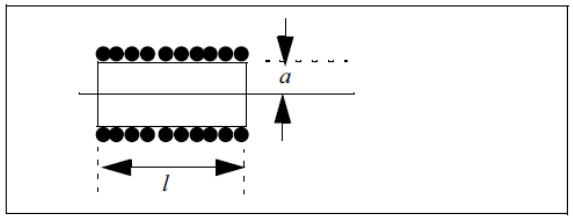
\includegraphics[scale=0.5]{antena/Bobina_N_Espiras.png}
\caption{Geometría de una bobina de N espiras.}
\label{fig:N_esp}
\end{figure}

La inductancia de una bobina depende, principalmente, de la geometría y el número de
espiras.

Según \cite{antena_AN710}, para calcular la inductancia L:

\begin{equation}
\boxed{L = \frac{(aN)^2}{22.9 a+25.4 l}}
\end{equation}

Donde a es el radio de la bobina, l es el largo, y N el número de espiras.\newline

\underline {Ejemplo:}\newline

Se desea calcular la inductancia de una bobina con las siguientes especificaciones.

\begin{itemize}
\item a = 25mm
\item l = 0.3mm N
\item N = 5
\end{itemize}

$$ L = \frac{(25mm*5)^2}{22.9*25mm+25.4*0.3mm*5}\mu Hy = 25.59 \mu Hy$$

\subsection{Cálculo del factor de calidad o selectividad Q}
El factor de calidad se calcula como:

\begin{equation}
\boxed{Q =\frac{\omega L}{R_{ac}}}
\end{equation}
\newline
\underline{Ejemplo:}\newline
Para los valores de L y R calculados anteriormente, hallar Q.

\begin{itemize}
\item L = 25.59 \mu Hy
\item $R_{ac}$ = 0.75 \Omega
\item \omega = 2\pi *13.56MHz
\end{itemize}

$$ Q = \frac{2\pi *13.56MHz*25.59\mu Hy}{0.75 \Omega} = 1907 $$

\subsubsection{Mediciones del solenoide de 5 espiras}
Se fabricó una antena con las características mencionadas al principio de la guía, y se midió
con un medidor RLC (Tonghui TH2826A). Luego se contrastaron los valores con un Qmetro
analógico.

\begin{figure}[H]
\centering
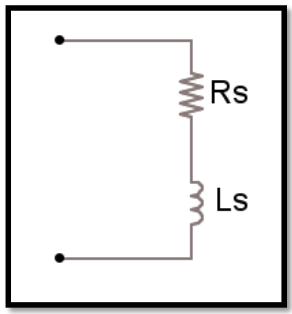
\includegraphics[scale=0.5]{antena/Equivalente_Bobina_Serie.png}
\caption{Circuito equivalente del inductor real.}
\label{fig:L_real}
\end{figure}


Se obtuvieron los siguientes datos:

\begin{table}[H]
\centering
\caption{Mediciones de la Antena}
\label{table:med_antena}
\begin{tabular}{c|c|c|c}
\textbf{Frecuencia [Hz]} & \textbf{Ls [Hy]}       & \textbf{Rs [\Omega]} & \textbf{Q}                                                                                \\ \hline
1000                    & 2.9039E-06 & 0.2648   & 0.06890291                                                                             \\
2000                 & 3.3124E-06 & 0.278   & 0.14972785                                                                             \\
100000                  & 3.2564E-06 & 0.2776   & 7.37061094                                                                                 \\
200000                  & 3.2404E-06 & 0.3012   & 13.5193621                                                                             \\
500000                  & 3.2262E-06 & 0.374   & 27.0998486                                                                             \\
800000                  & 3.1978E-06 & 0.4432   & 36.2680427                                                                             \\
1000000                  & 3.1899E-06 & 0.4705   & 42.598928                                                                             \\
200000                  & 3.0715E-06 & 0.7688   & 50.2041871          
\end{tabular}
\end{table}

\begin{figure}[H]
\centering
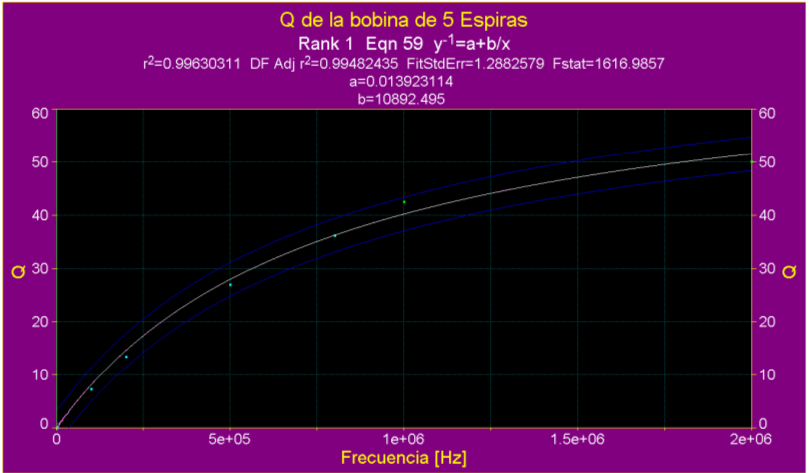
\includegraphics[scale=0.5]{antena/Simulacion_Q_Antena.png}
\caption{Variación del Q de la bobina con la frecuencia.}
\label{fig:L_Qsim}
\end{figure}

Ajustando la curva, vemos que la Q varía aproximadamente de la siguiente forma:

$$ Q = \frac{1}{a + \frac{b}{f}} = \frac{1}{0.0139 + \frac{10892.495}{f}} $$

Para la frecuencia de interés (f = 13.56 MHz):
$$Q = 67.90528 \pm 3.152254 \textrm{      ;con un intervalo de confianza del 95\%} $$ 

\subsection{Antena para testing}
Tomándose como base las normas de testeo ISO/IEC10373 \cite{nfc_test} se realizó la fabricación de una antena para las pruebas de laboratorio del circuito integrado \ref{fig:L_test}.
La inductancia mostrada por esta antena fue
de 1,6 μHy, obteniendo, para una resonancia a
13,56 MHz, una capacidad paralela necesaria de
88 pF.



\begin{figure}[H]
\centering
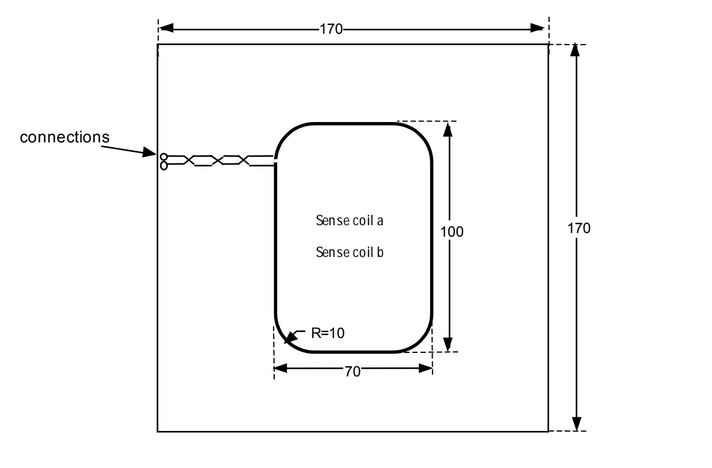
\includegraphics[scale=0.6]{antena/Bobina_Testing.JPG}
\caption{Antena para testing (ISO/IEC10373).}
\label{fig:L_test}
\end{figure}




